Technical Coordination (TC) is responsible for detector integration
and installation support. 
%The technology for massive noble liquid detectors has developed over the last \num{45} years and the first large \dword{lartpc} was completed in 2010. While multiple \dwords{lartpc} have operated worldwide, the technology is still relatively new and the scale up to \dword{dune} presents challenges. However, the technology is well suited to massive neutrino detectors with millimeter scale resolution on \SI{100}{m} scale detectors and the technical challenges are surmountable.
The \dword{dune} collaboration consists of a large number of
institutions distributed throughout the world. They are supported by a
large number of funding sources and collaborate with a large number of
commercial partners. Groups of institutes within \dword{dune} form
consortia that take complete responsibility for construction of their
system.  \dword{dune} has empowered several consortia (currently nine)
with the responsibility to secure funding and design, fabricate,
assemble, install, commission and operate their components of the
\dword{dune} \dword{fd}. There are three consortia focusing
exclusively on the single phase detector: anode plane assembly (APA),
cold electronics (SPCE) and photon detector (SPPD). There are three
focusing exclusively on the dual phase detector: charge readout plane
(CRP), cold electronics (DPCE) and photon detector (DPPD). There are
three joint consortia: high voltage (HV), data acquisition (DAQ) and
cryogenic instrumentation and slow control (CISC). Other consortia may
be formed over time as concepts more fully emerge, such as a
\dword{fd} calibration system and various aspects of the \dword{nd}.
\dword{dune} Technical Coordination, under the direction of the
\dword{dune} Technical Coordinator, has responsibility to monitor the
technical aspects of the detector construction, to integrate and
install the detector and to deliver the common projects. The
\dword{dune} TC organization is shown in Fig.~\ref{fig:TC_orgchart}.
\begin{figure}[htb]
  \begin{center}
    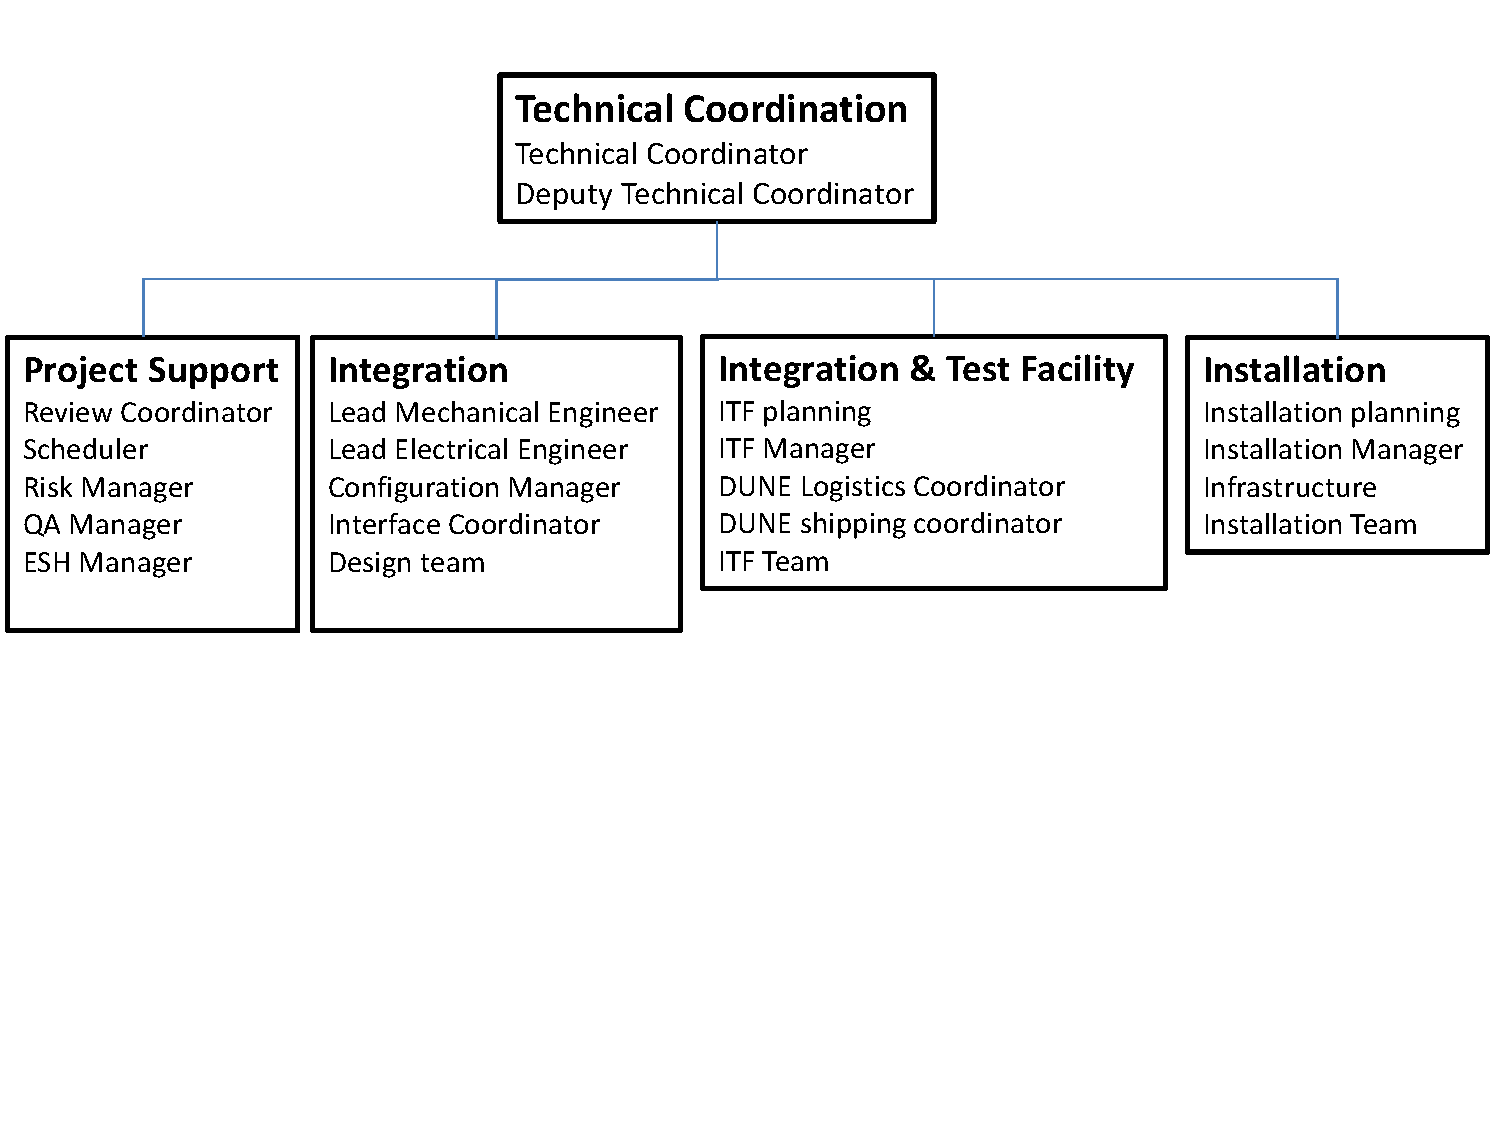
\includegraphics[width=\textwidth]{far-detector-generic/figures/TP_TC_Org_Chart}
    \caption{Organization of Technical Coordination. This organization
      oversees the construction of the \dword{fd}, both single and
      dual phase, and the \dword{nd}.}
    \label{fig:TC_orgchart}
  \end{center}
\end{figure}
The TC organization staffing will grow over time as the project
advances. TC will provide staffing for teams underground at SURF, at
integration facilities and at the near site at FNAL, in addition to
the core team distributed among collaborating institutions.

The \dword{dune} Project consists of a \dword{fd} and a
\dword{nd}. The \dword{nd} is at a pre-conceptual state; as the
Conceptual Design and organization emerges, it will become part of the
\dword{dune} Project. Currently the \dword{dune} Project consists of
the \dword{dune} \dword{fd} consortia and Technical Coordination.  The
\dword{dune} Project is moving towards a Technical Design Report for
the \dword{fd}, both single and dual phase options, in 2019. It is
expected that a Conceptual Design Report for the \dword{nd} will be
prepared at the same time. \dword{fd} components will be shipped
from the consortia construction sites to the the \dword{itf}. TC will
evaluate and accept consortia components either at integration
facilities or the installation site and oversee the integration of
components as appropriate. The scope of the \dword{fd} integration
and installation effort is shown graphically in
Fig.~\ref{fig:TC_flow}.
\begin{figure}[htb]
  \begin{center}
    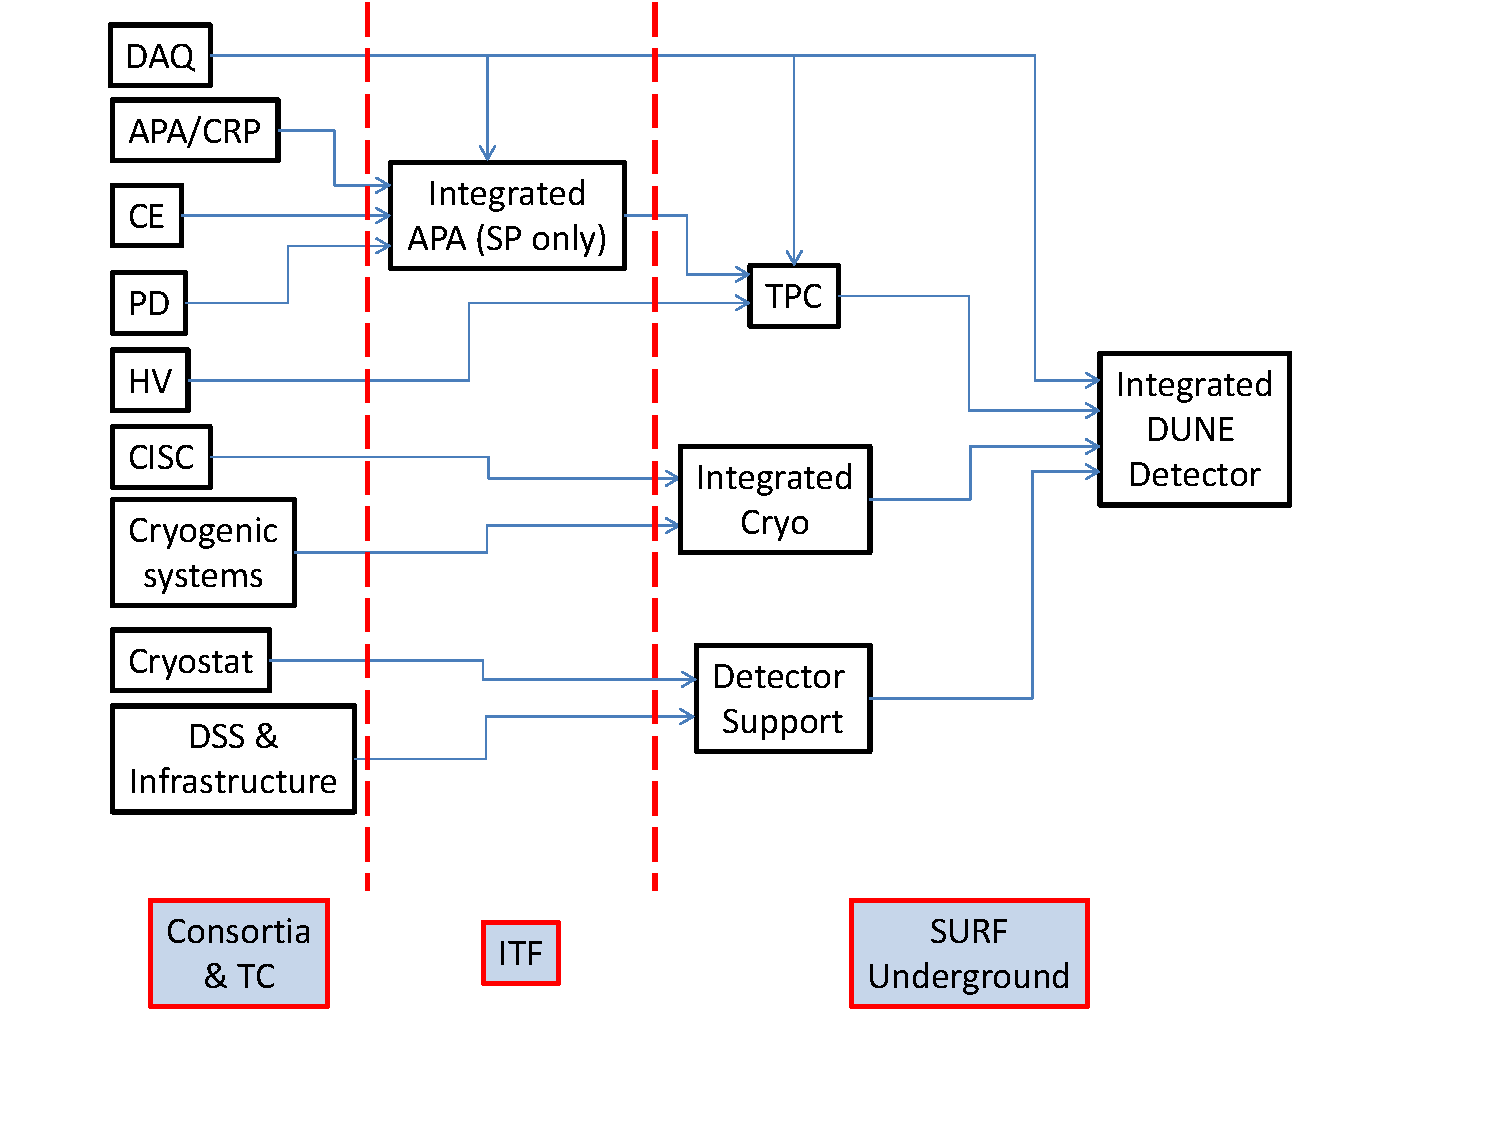
\includegraphics[width=\textwidth]{far-detector-generic/figures/DUNE_deliverable_flow}
    \caption{Flow of components from the consortia to the \dword{fd}.}
    \label{fig:TC_flow}
  \end{center}
\end{figure}

TC interacts with the consortia via three main areas: project
coordination, integration and installation.  Construction of the
\dword{dune} Detector requires careful technical coordination due to
its complexity.  Given the horizontal nature of the consortia
structure and the extensive interdependencies between the systems, a
significant engineering organization is required to deliver
\dword{dune} on schedule and within specifications and funding
constraints.

The responsibilities of Technical Coordination include:
\begin{itemize}
  \item management and delivery of all common projects
  \item development and monitoring of the consortia interfaces
  \item configuration control of all interface documents, drawings and envelopes
  \item installation of detectors at the near and far sites
  \item logistics for detector integration and installation at the near and far sites
  \item survey of the detector
  \item primary interface to \dword{lbnf} for conventional facilities, cryostat and cryogenics
  \item primary interface to the Host Lab for infrastructure and operations support
  \item development and tracking of project schedule and milestones
  \item review of all aspects of the project
  \item recording and approving all project engineering information, including: documents, drawings and models
  \item project work breakdown schedules
  \item project risk register
  \item \dword{dune} engineering and safety standards, including grounding \& shielding
  \item monitoring of all consortia design and construction progress
  \item quality assurance and all QA related studies and documents
  \item \dword{esh} organization and all safety related studies and documents
\end {itemize}

\dword{dune} TC interacts with \dword{lbnf} primarily through the
\dword{lbnf}/\dword{dune} systems engineering organization. TC
provides the points of contact between the consortia and \dword{lbnf}.
TC will work with the \dword{lbnf}/\dword{dune} Systems Engineer to
implement the \dword{lbnf}/\dword{dune} Configuration Management Plan
to assure that all aspects of the overall \dword{lbnf}/\dword{dune}
project are well integrated. TC will work with \dword{lbnf} and the
Host Lab to ensure that adequate infrastructure and operations support
are provided during construction, integration, installation,
commissioning and operation of the detectors. The LBNF/DUNE systems
engineering organization is shown in Fig.~\ref{fig:DUNE_SE_org}.
\begin{figure}[htb]
  \begin{center}
    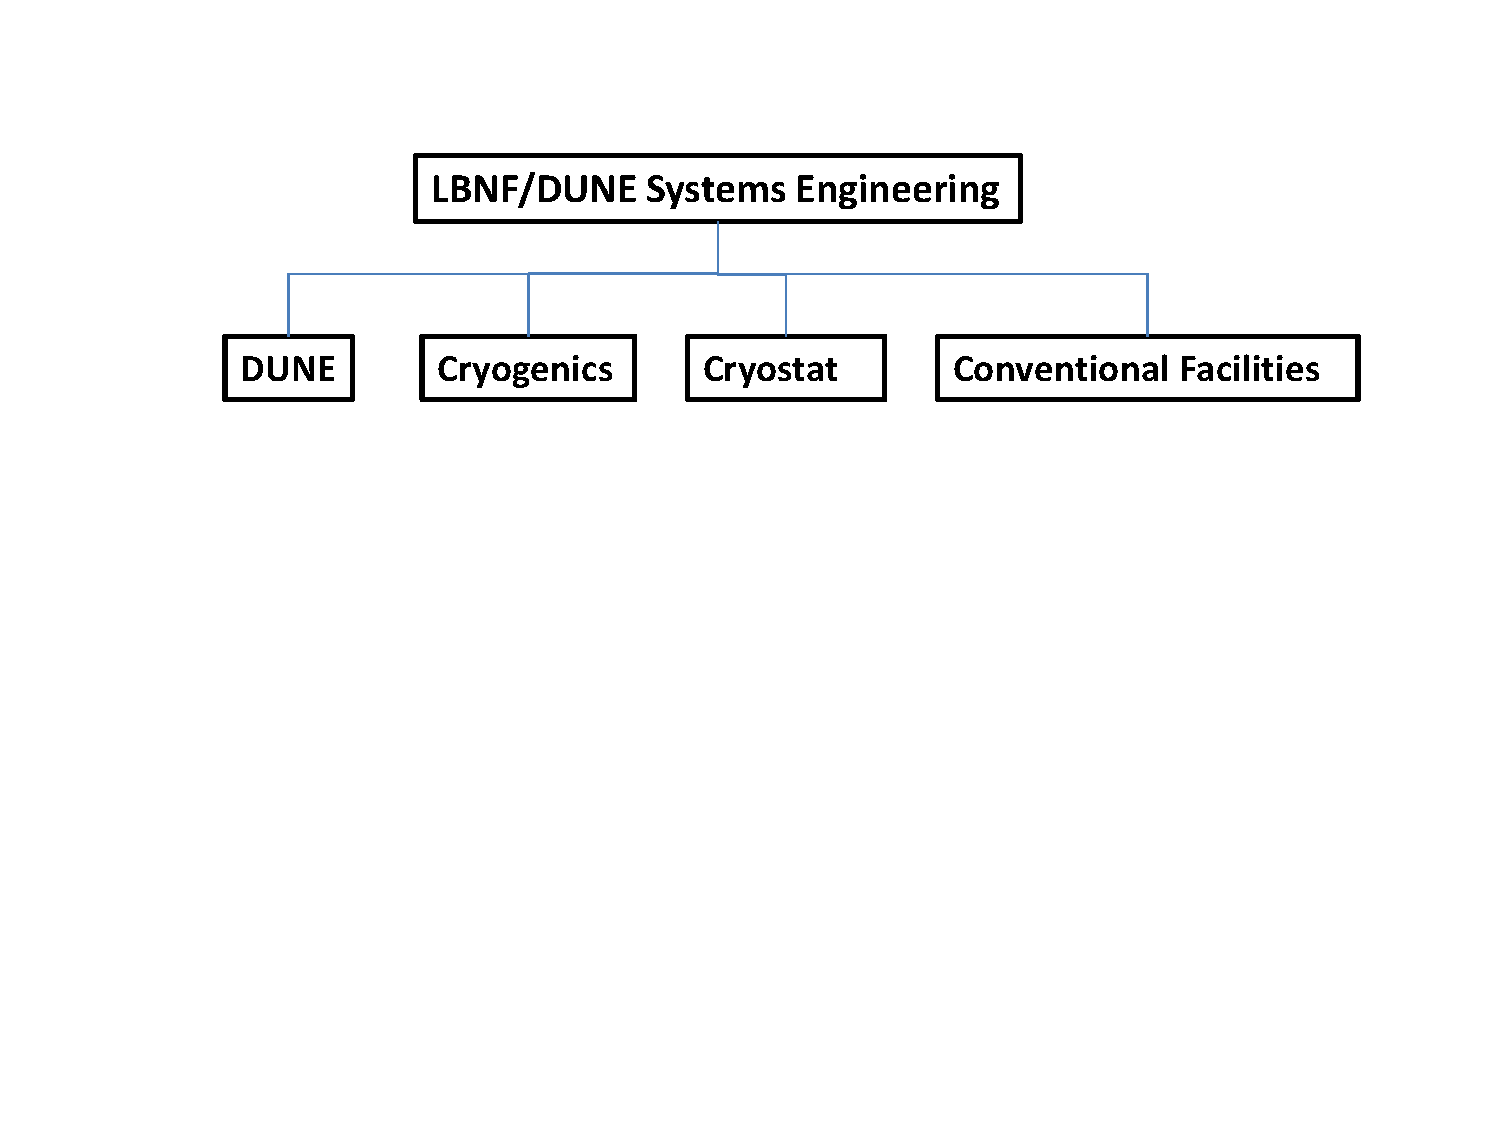
\includegraphics[width=\textwidth]{far-detector-generic/figures/TC_SE_Org_Chart}
    \caption{LBNF/DUNE systems engineering organizational structure.}
    \label{fig:DUNE_SE_org}
  \end{center}
\end{figure}
Proper integration of the \dwords{fd} within the supporting
facilities and infrastructure at SURF is a major engineering task.
The \dword{lbnf}/\dword{dune} Systems Engineer is responsible for the
interfaces between the major \dword{lbnf} and \dword{dune} systems
(conventional facilities, cryostats, cryogenics systems and
detectors). The \dword{lbnf}/\dword{dune} systems engineering team
includes several engineers and designers with responsibility for
maintaining computer aided design (CAD) models. \dword{dune} TC
supports an engineering team that works directly with the
\dword{lbnf}/\dword{dune} systems engineering team to ensure that the
detector is properly integrated into the overall system.

TC has been working with the LBNF/DUNE systems engineering team to
define requirements from DUNE for the conventional facilities final
design for the detector chambers, central utility cavern (CUC), drifts
and utilities. TC is representing the interests of the DUNE detector
in the conventional facilities (CF) design. This includes refining the
detector installation plan to understand how much space is needed in
front of the temporary construction openings (TCO) of the cryostats
and therefore of the size of the chambers. TC continues to refine the
detector needs for utilities in the detector caverns and the central
utility cavern where the DAQ will be housed.

Physics requirements on TC include cleanliness in the cryostats,
survey and alignment tolerances and grounding \& shielding
requirements. The cleanliness requirement is for ISO 8 (class
100,000), which will keep rates from dust radioactivity below those of
the inherent $^{39}$Ar background. The alignment tolerances are driven
by physics requirements on reconstructing tracks. Grounding and
shielding is critical to enable this very sensitive, low noise
detector to achieve the required signal to noise. The physics
requirements for \dword{lbnf} and \dword{dune} are maintained in
DocDB.
